\documentclass[11pt]{report}
\usepackage{geometry}
\geometry{letterpaper, top=1in, bottom=1in, left=1in, right=1in}                                 
\usepackage[parfill]{parskip}   
\usepackage{graphicx}
\usepackage{amssymb}
\usepackage{epstopdf}
\usepackage{array}
\usepackage{tabularx}
\usepackage{hyperref}
\hypersetup{
    colorlinks=true,
    linkcolor=blue,
    filecolor=magenta,      
    urlcolor=cyan
    }


\setlength{\parindent}{0em}
\pagenumbering{gobble}

\DeclareGraphicsRule{.tif}{png}{.png}{`convert #1 `dirname #1`/`basename #1 .tif`.png}

\newcommand{\newday}[1]{\newpage{\LARGE \textbf{#1}}\\}
\newcommand{\imagefolder}{/Users/lauriaclarke/Documents/mfadt/ms1/lauriaclarke.github.io/instructionsetsforstrangers}


\title{{\LARGE\textbf{7 in 7}} \\ (all the photos are in the images directory, just haven't had time to place them properly in the document)}
\date{\today}
%\author{}
                                   
\begin{document}
\maketitle
%\tableofcontents
%----------------------------------------------
\clearpage
\subsection*{five (11/03/2021)}
\textbf{name:} brainmelting openscad brachea exercise

\textbf{soundtrack:} Palomino by Trampled by Turtles then Norman Fucking Rockwell by Lana Del Rey 

The intent of this prototype was to model a breachea in 3D for printing. I did a lot of thinking at work today and was not prepared to think more. Luckily, David, my brain multiplier was available. This is as far as I got.
\begin{figure}[h]
\centering
  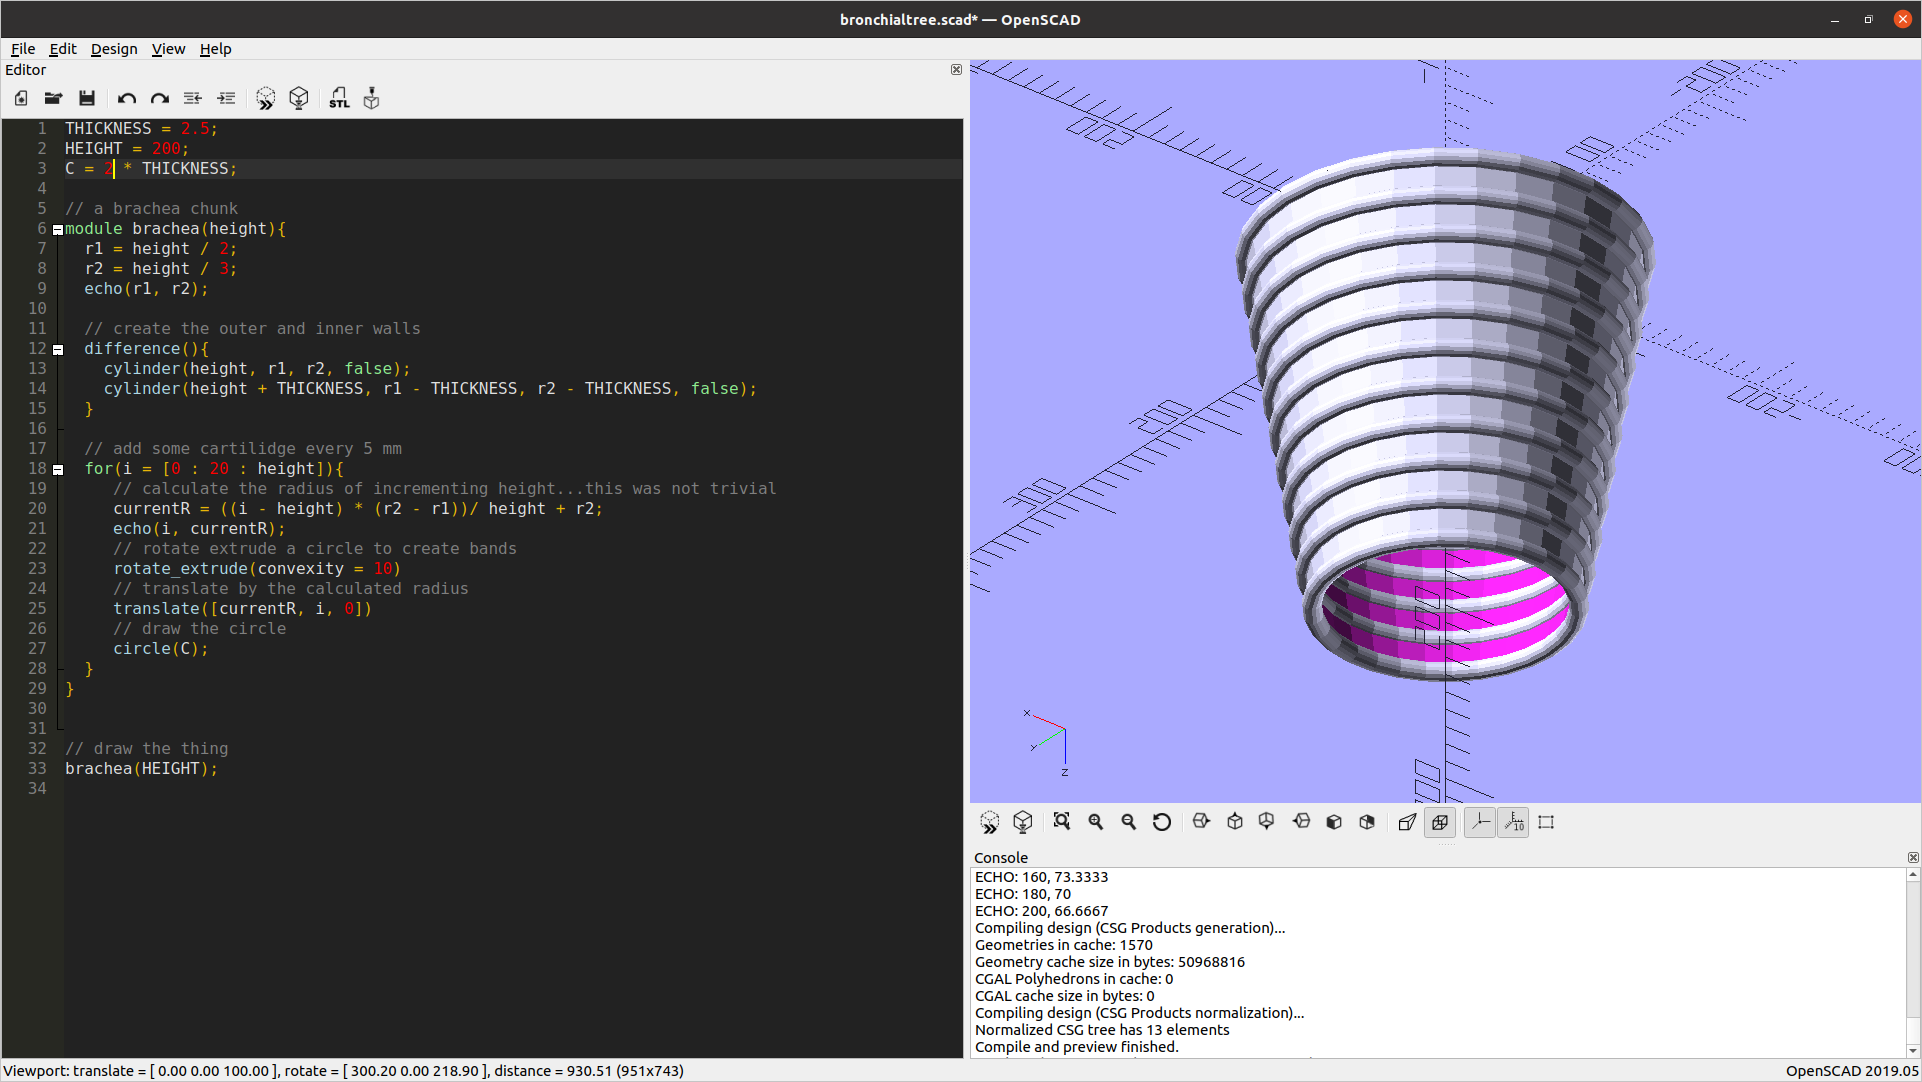
\includegraphics[width=\textwidth]{images/53.png}
  \caption{the beginning of a 3d model}
\end{figure}




\clearpage
\subsection*{five (11/03/2021)}
\textbf{name:} trachea support trial no. 1

\textbf{soundtrack:} Ice On The Dune by Empire of the Sun

The objective of this prototype was to create a mechanically robust way to actually make the trachea prototype move and such. First, I did some sketching and head scratching. Then I felt overwhelmed, but I kept thinking. I decided I needed a support on both the curved and flat sides of the trachea tube. One side would just act as support, while the other side allowed the monofillament to be pulled, causing the trachea to contract. After thinking through all kinds of unweidly solutions I had the idea to use pieces of dowel with small holes drilled through both to anchor the trachea and provide the pulling surface. 

So I put my shoes on and walked the 80 feet between my apartment and the hardware store -- this apartment is perfect in so many ways -- and got a 3/8" dowel for \$1.40. I measured out a length long enough to suspend the trachea and sit inside a piece of scrap wood and cut two pieces. 

Then I marked out where the holes should go; just in line with the vinyl tubing in the trachea. Next, I carefully punched and drilled some small holes through the dowel and added some 3/8" holes -- with a few different spacings -- to my scrap wood to seat the dowels.


The next step was tricky. I needed to create a way to anchor the curved side of the trachea to one of the dowels with holes in it. The catch being no glue was allowed (I alwyas try hard not to use glue when prototyping for maximum material resuse). After thinking for a while, I took a sewing needle and threaded it with monofilament. Then, I carefully pierced and went through the back of the curved side of each vinyl tube leaving about 4" of monofillaent on both sides of the hole. 

Finally, I was ready. Starting with the curved, anchor side, I attached one of the dowels to the trachea. Then I seated the anchor dowel in my scrap wood and threaded the other side through the holes. Tying knots in monofillament is always fiddly. The final result looked pretty cool 

Then I got to play with it! Wow, it worked better than anticipated!

\begin{figure}[h]
\centering
  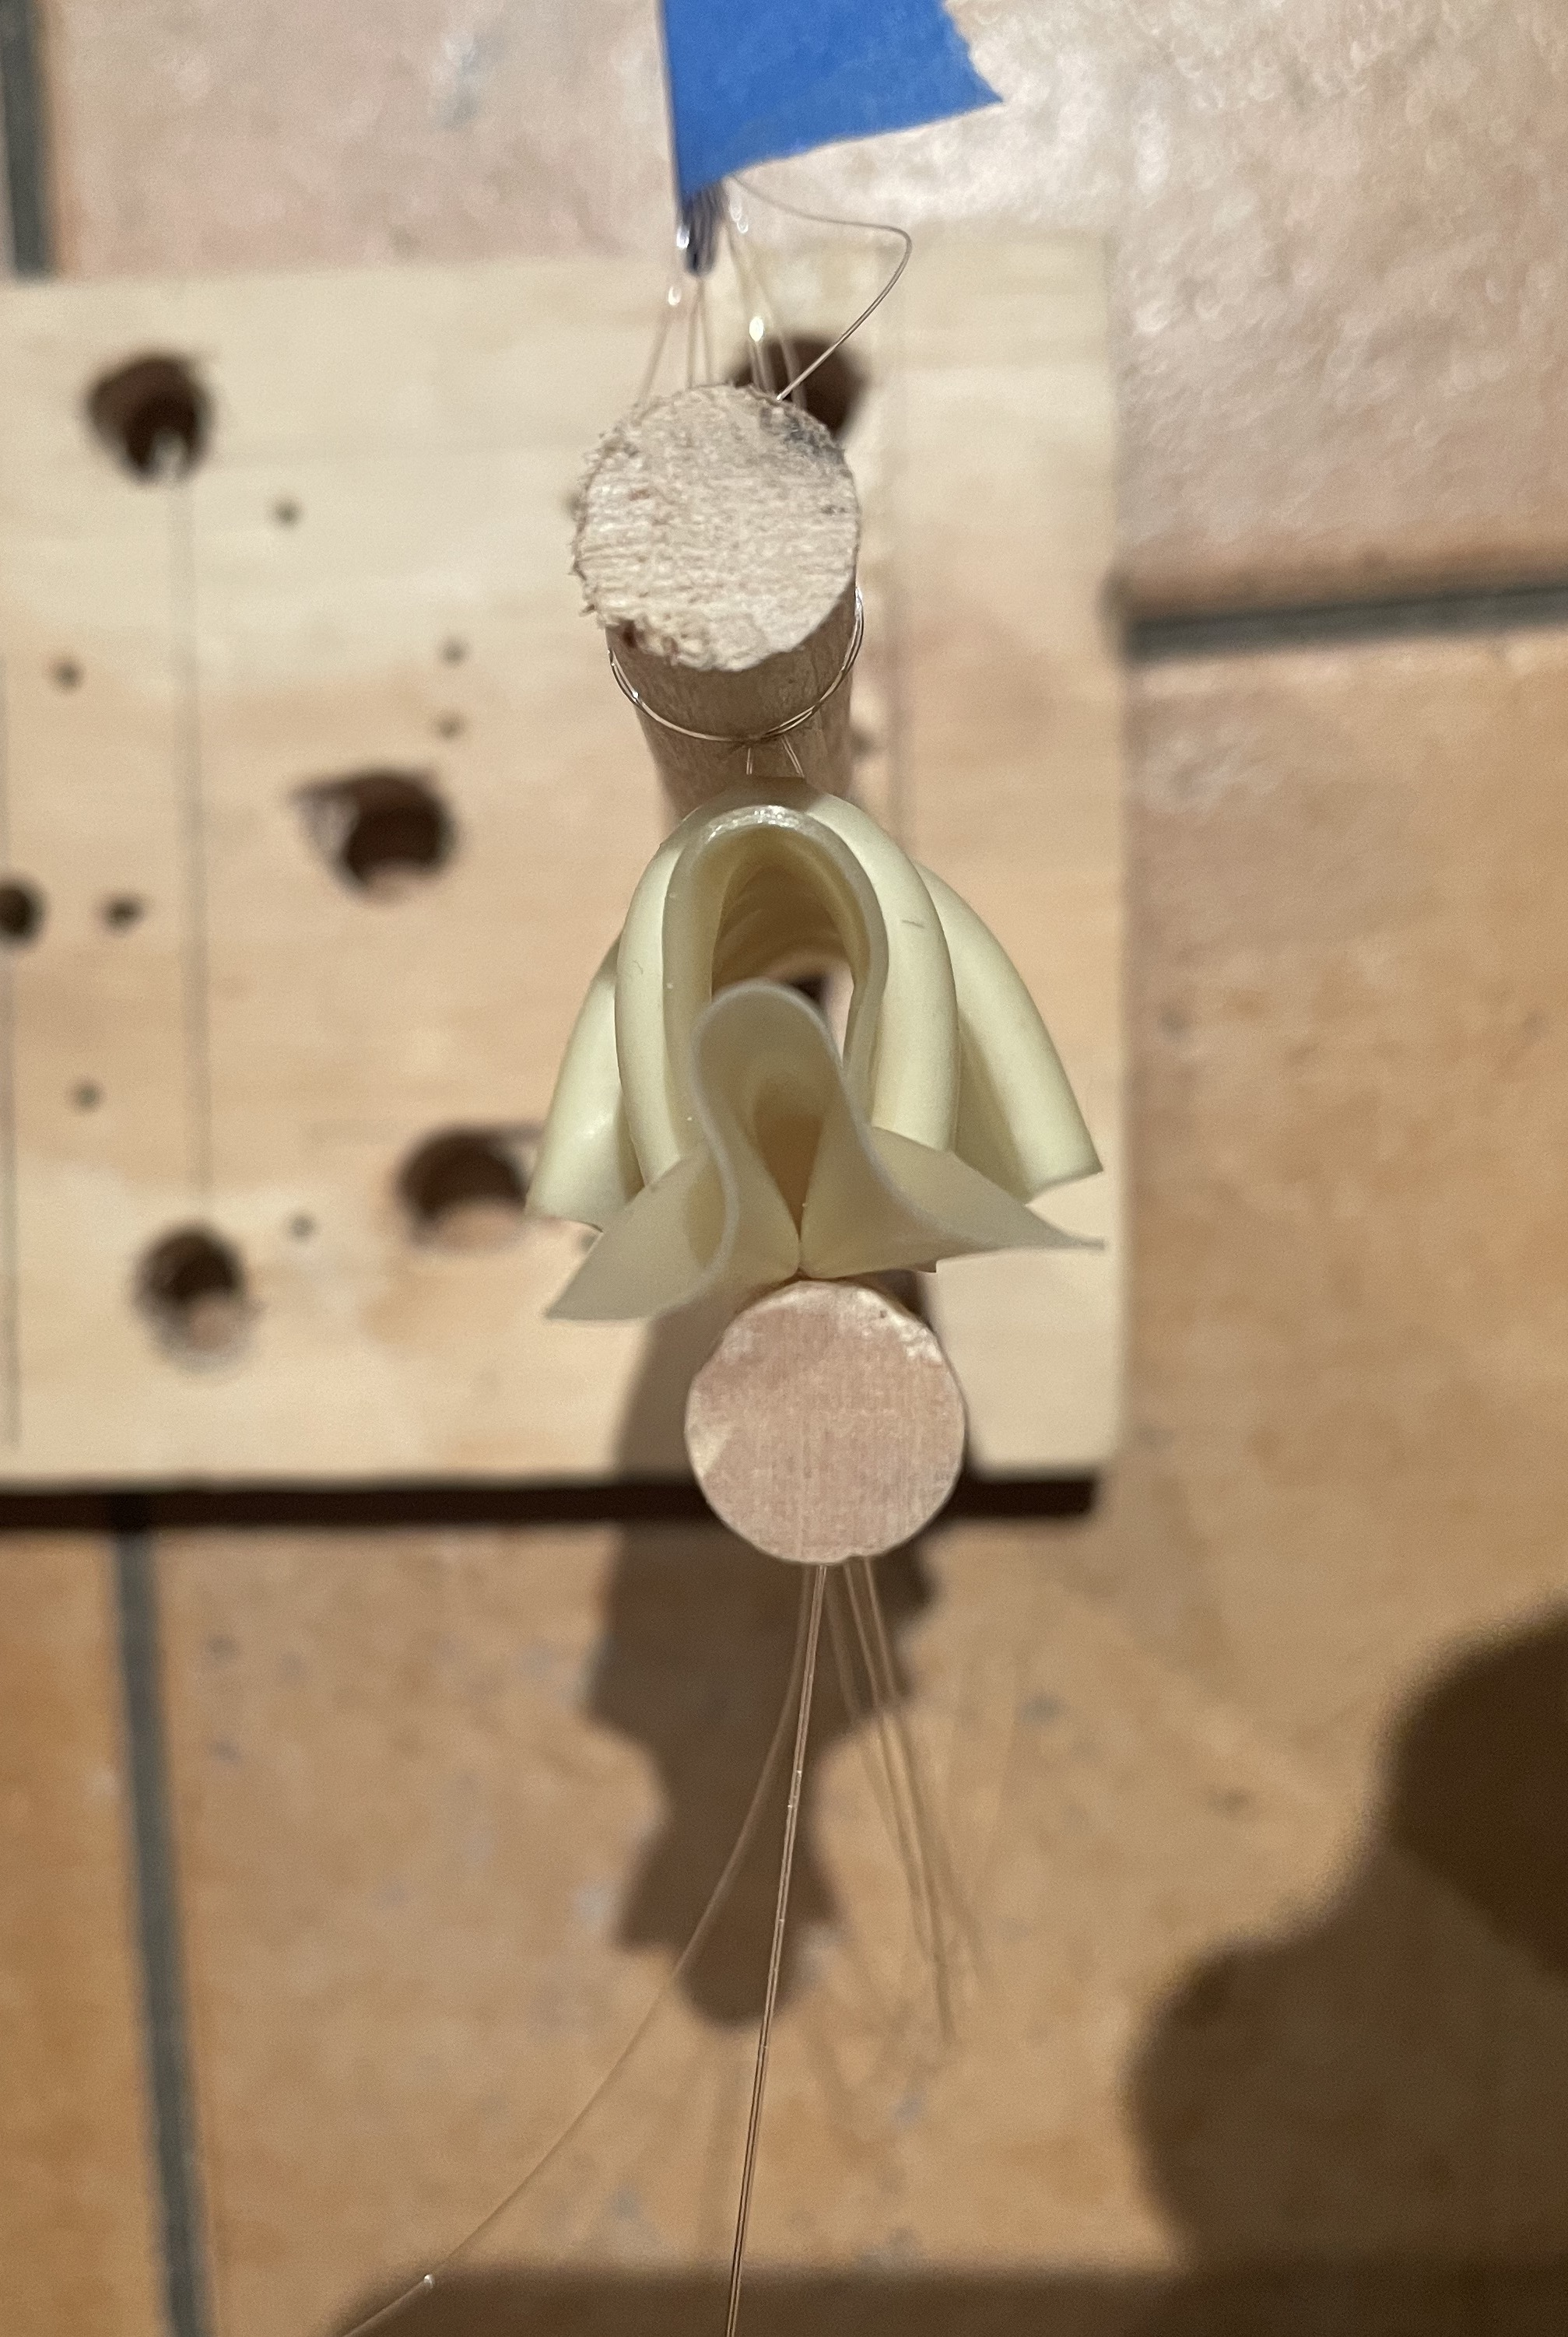
\includegraphics[width=0.22\textwidth]{images/46.JPG}
  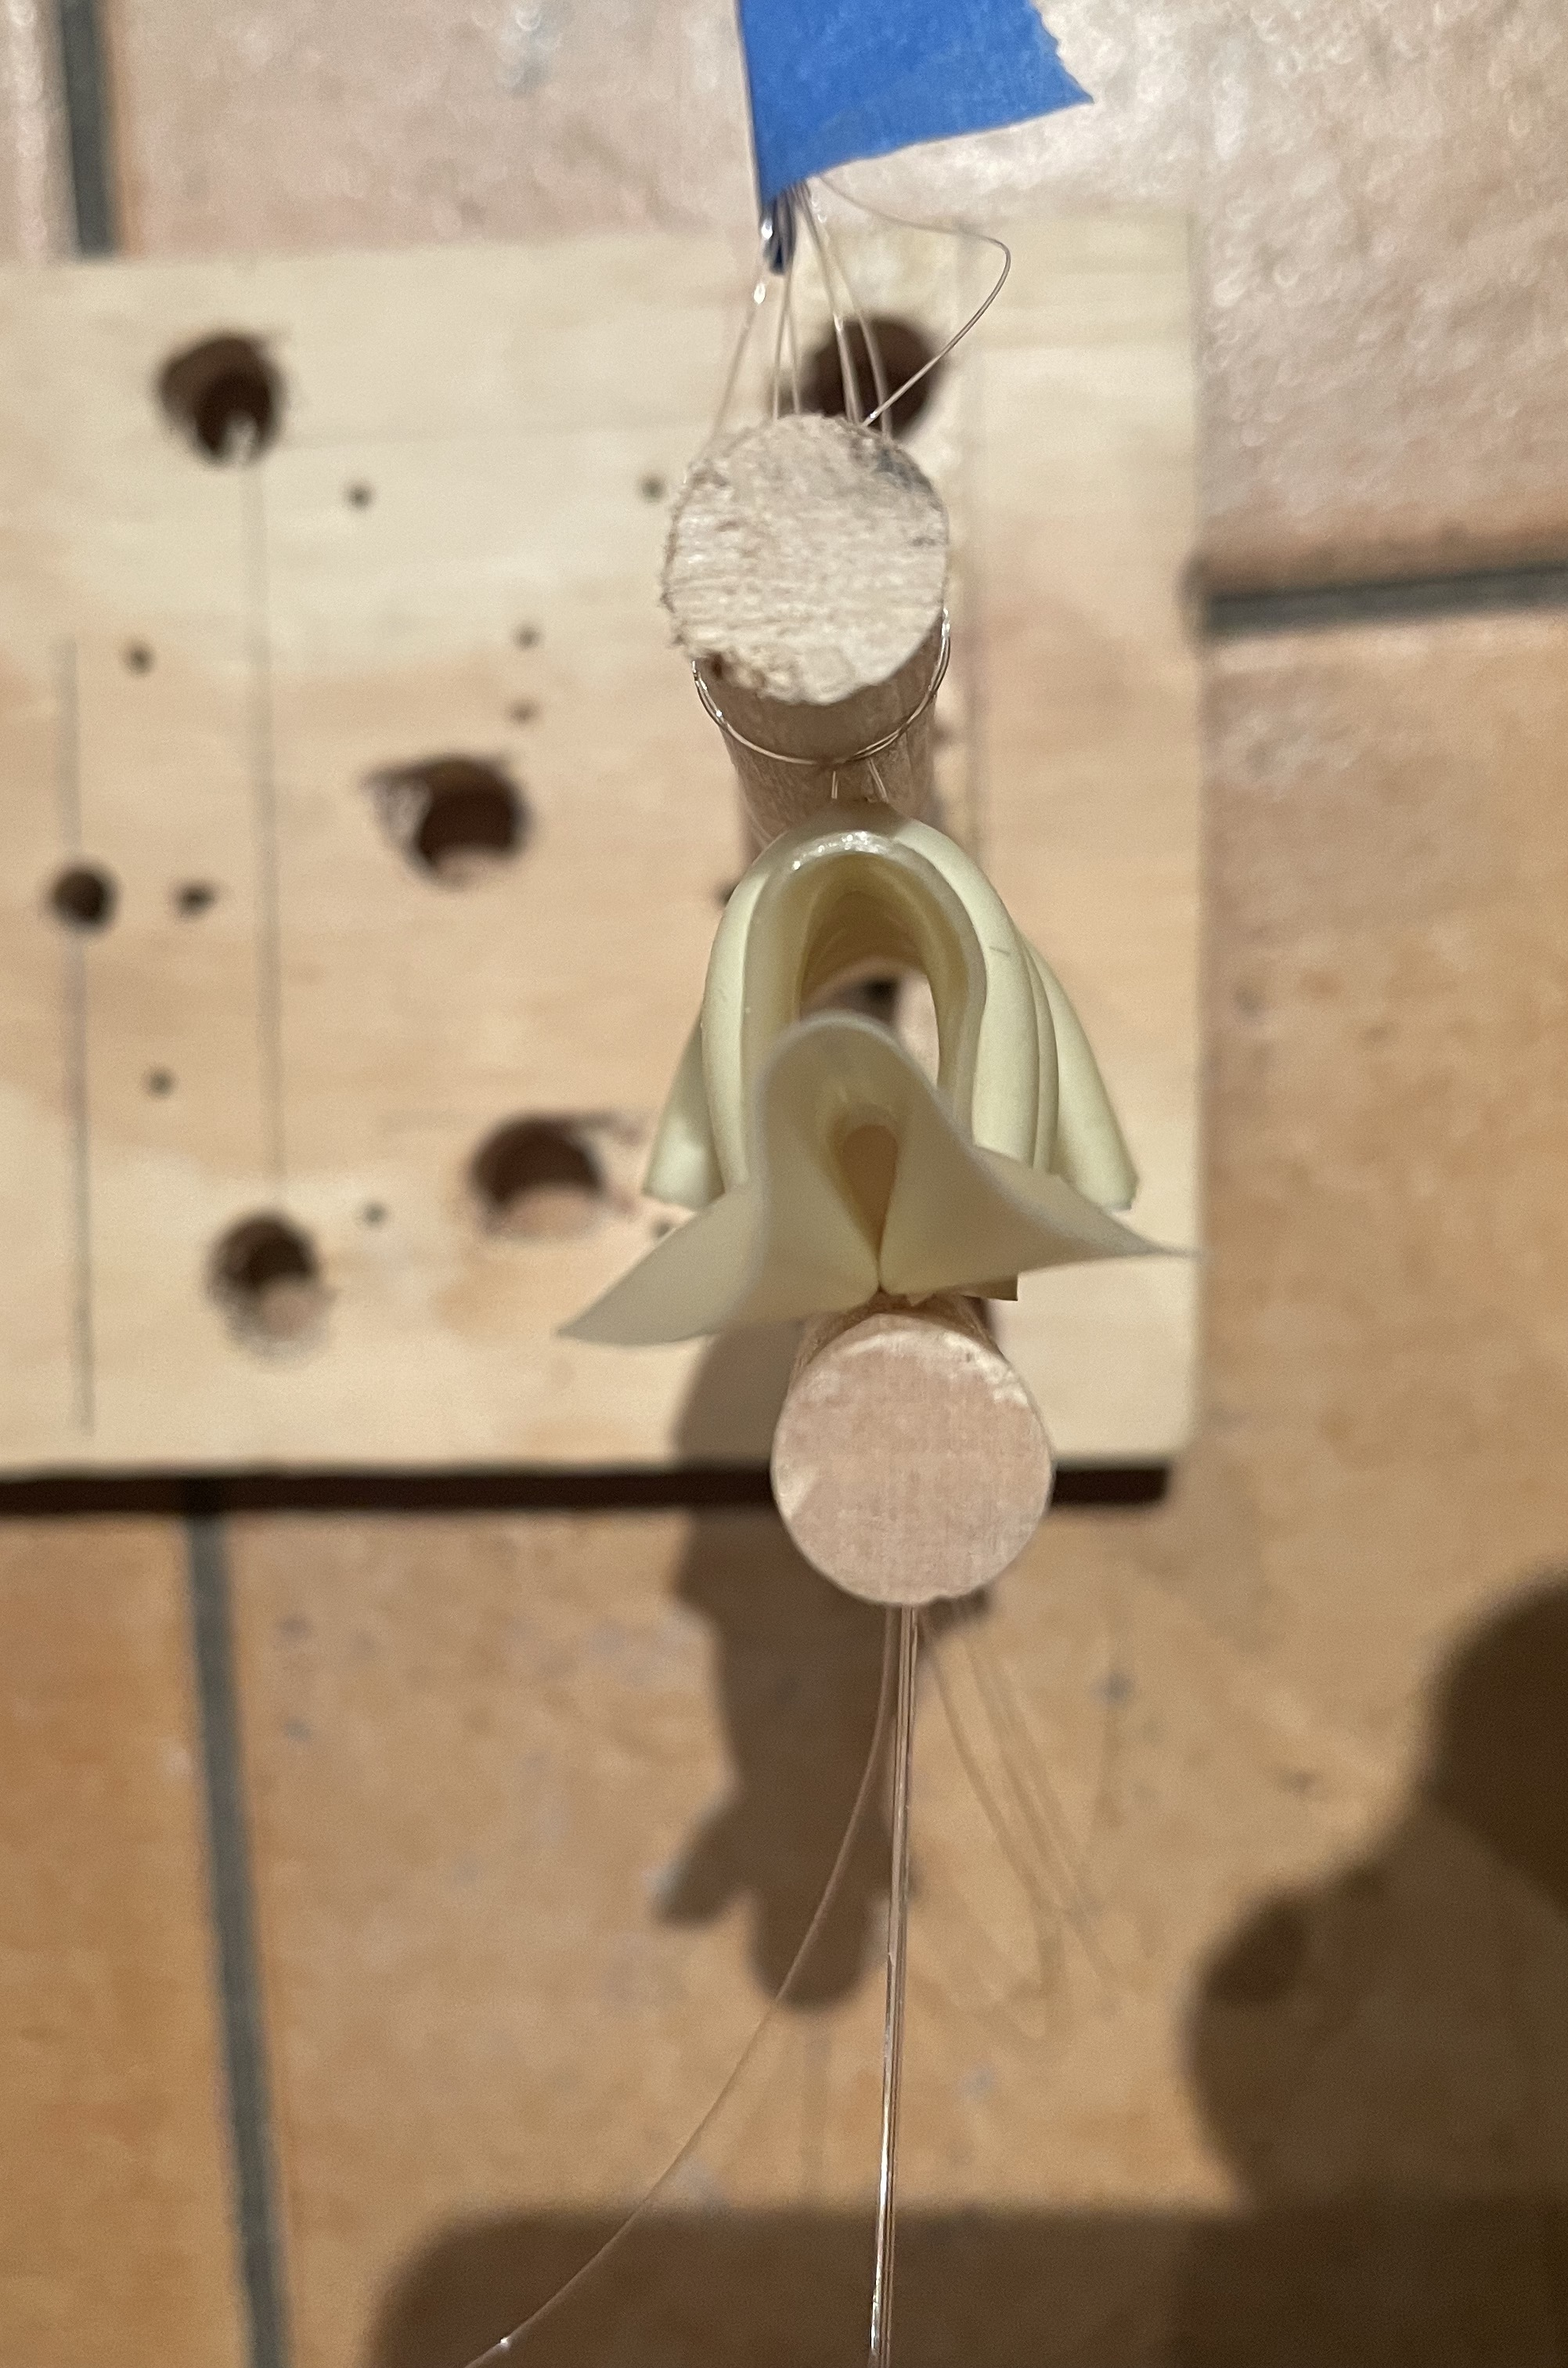
\includegraphics[width=0.22\textwidth]{images/47.JPG}
  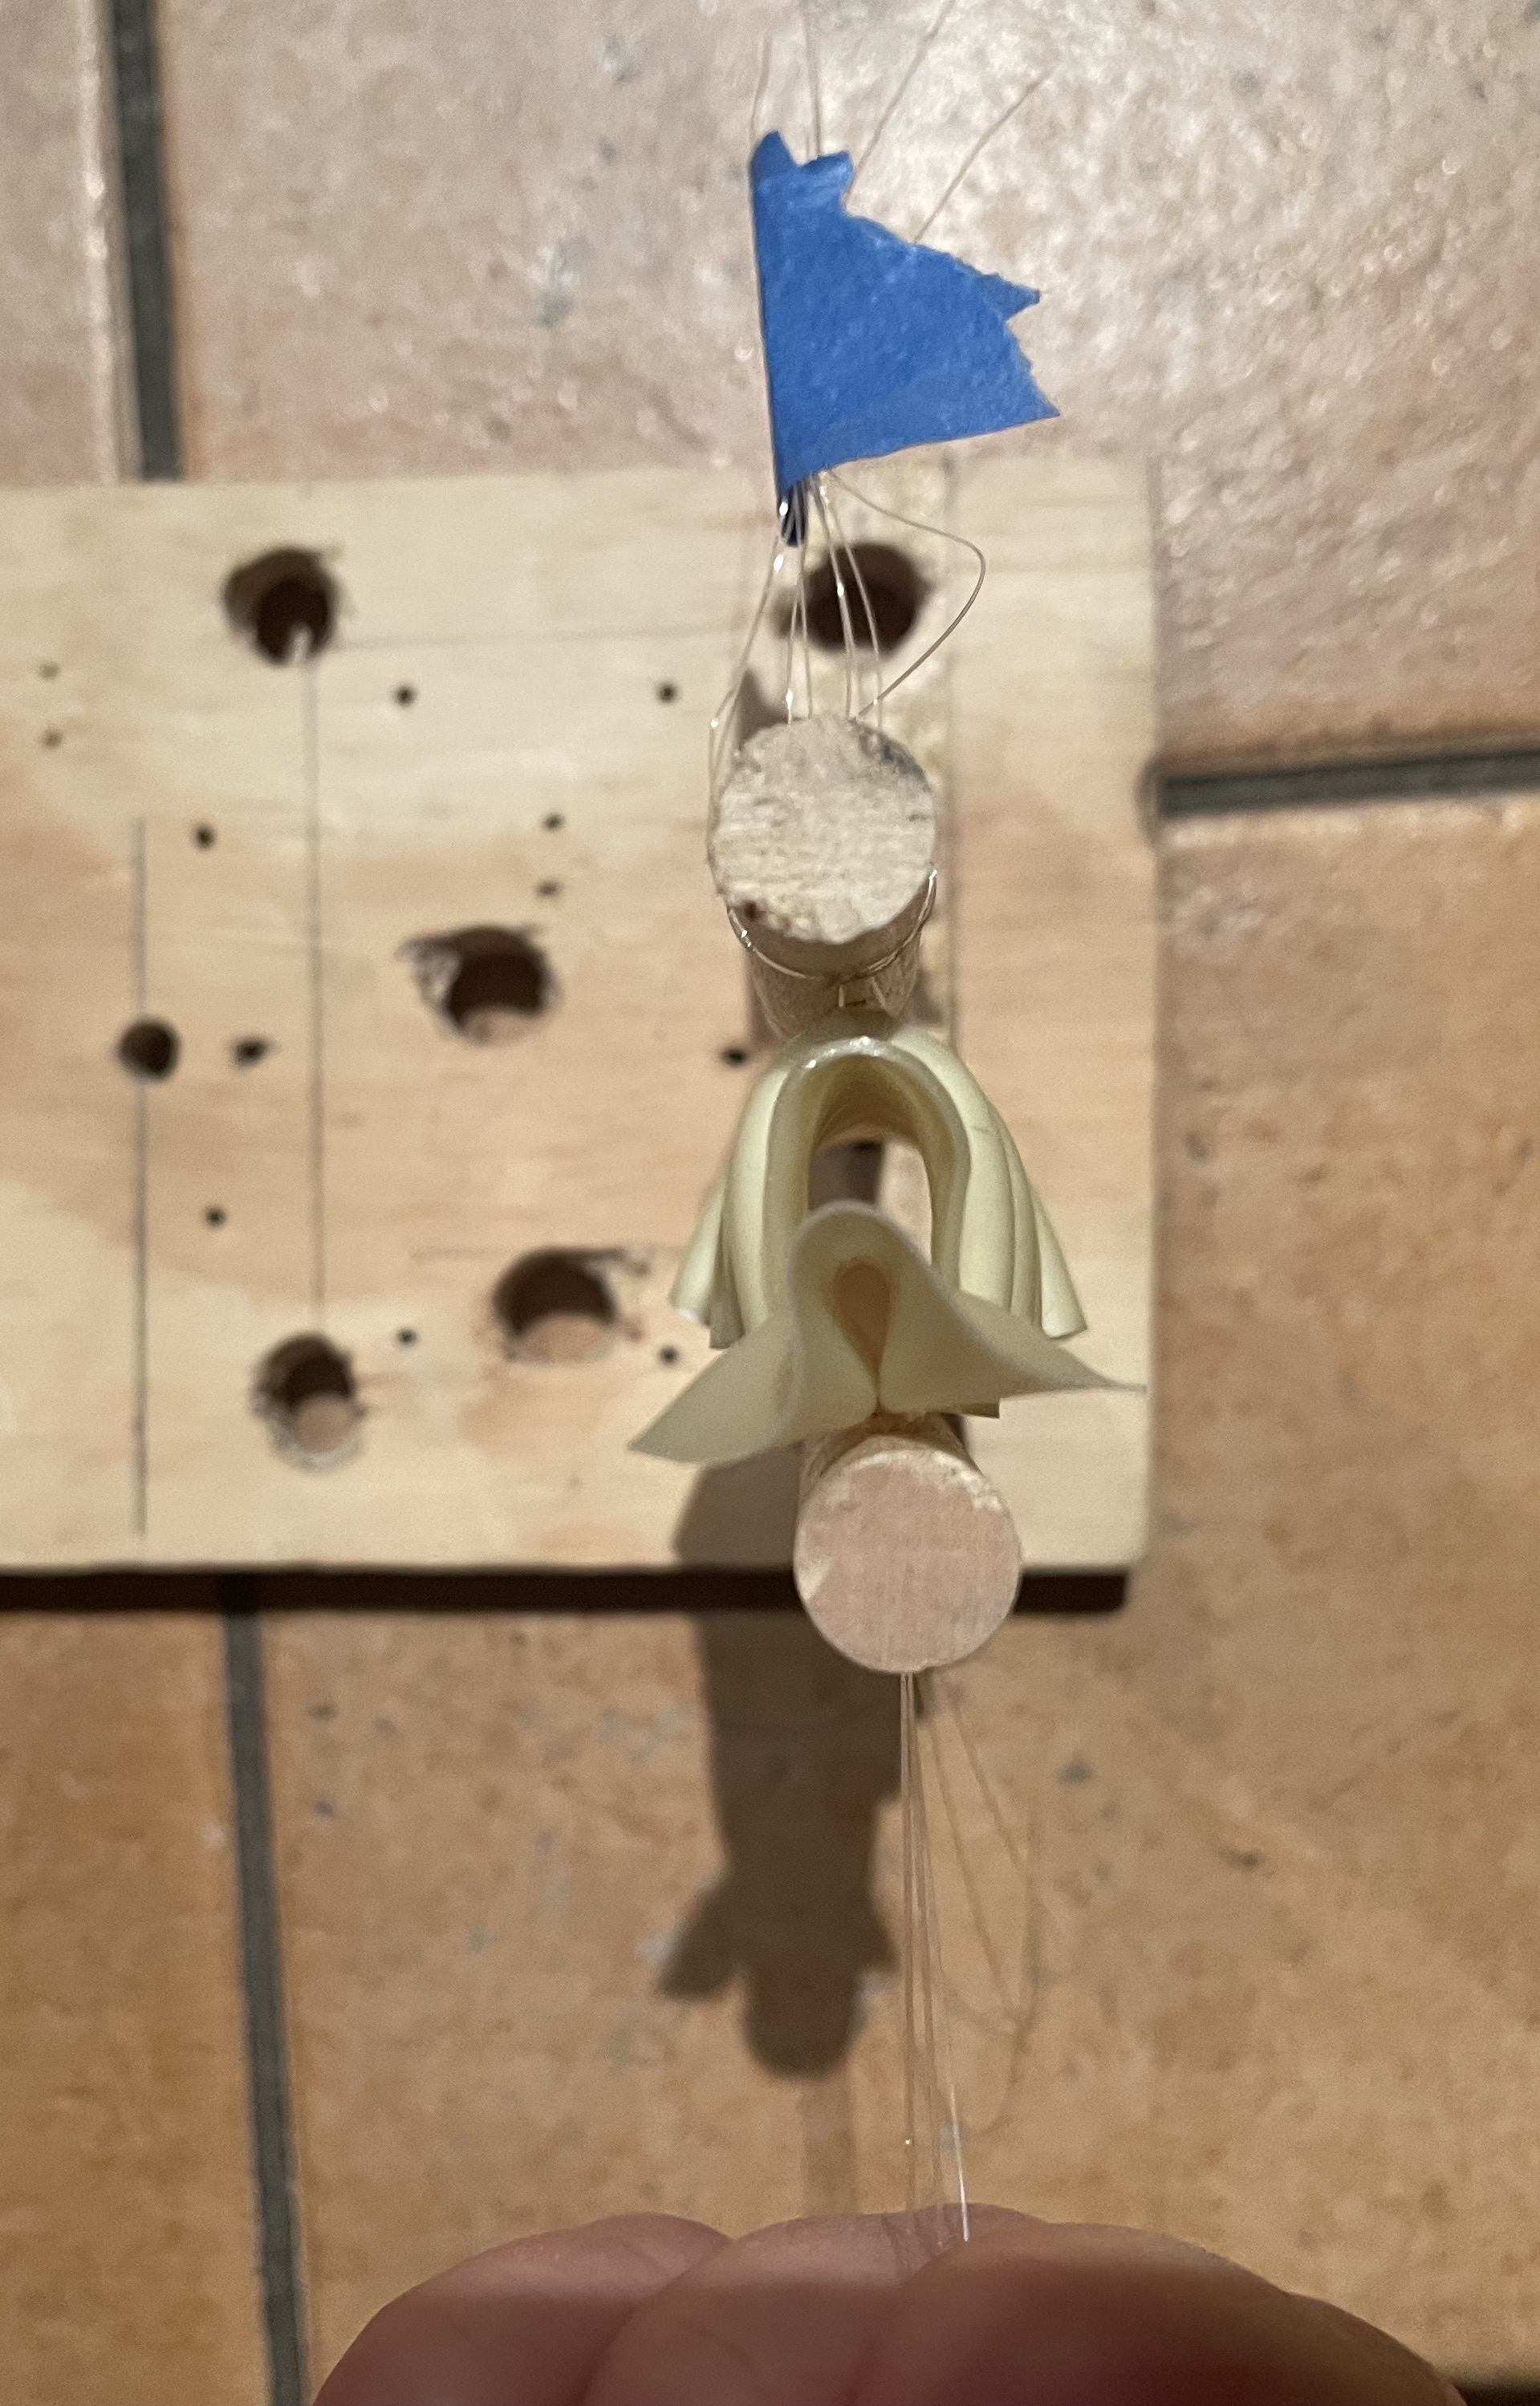
\includegraphics[width=0.22\textwidth]{images/48.JPG}
  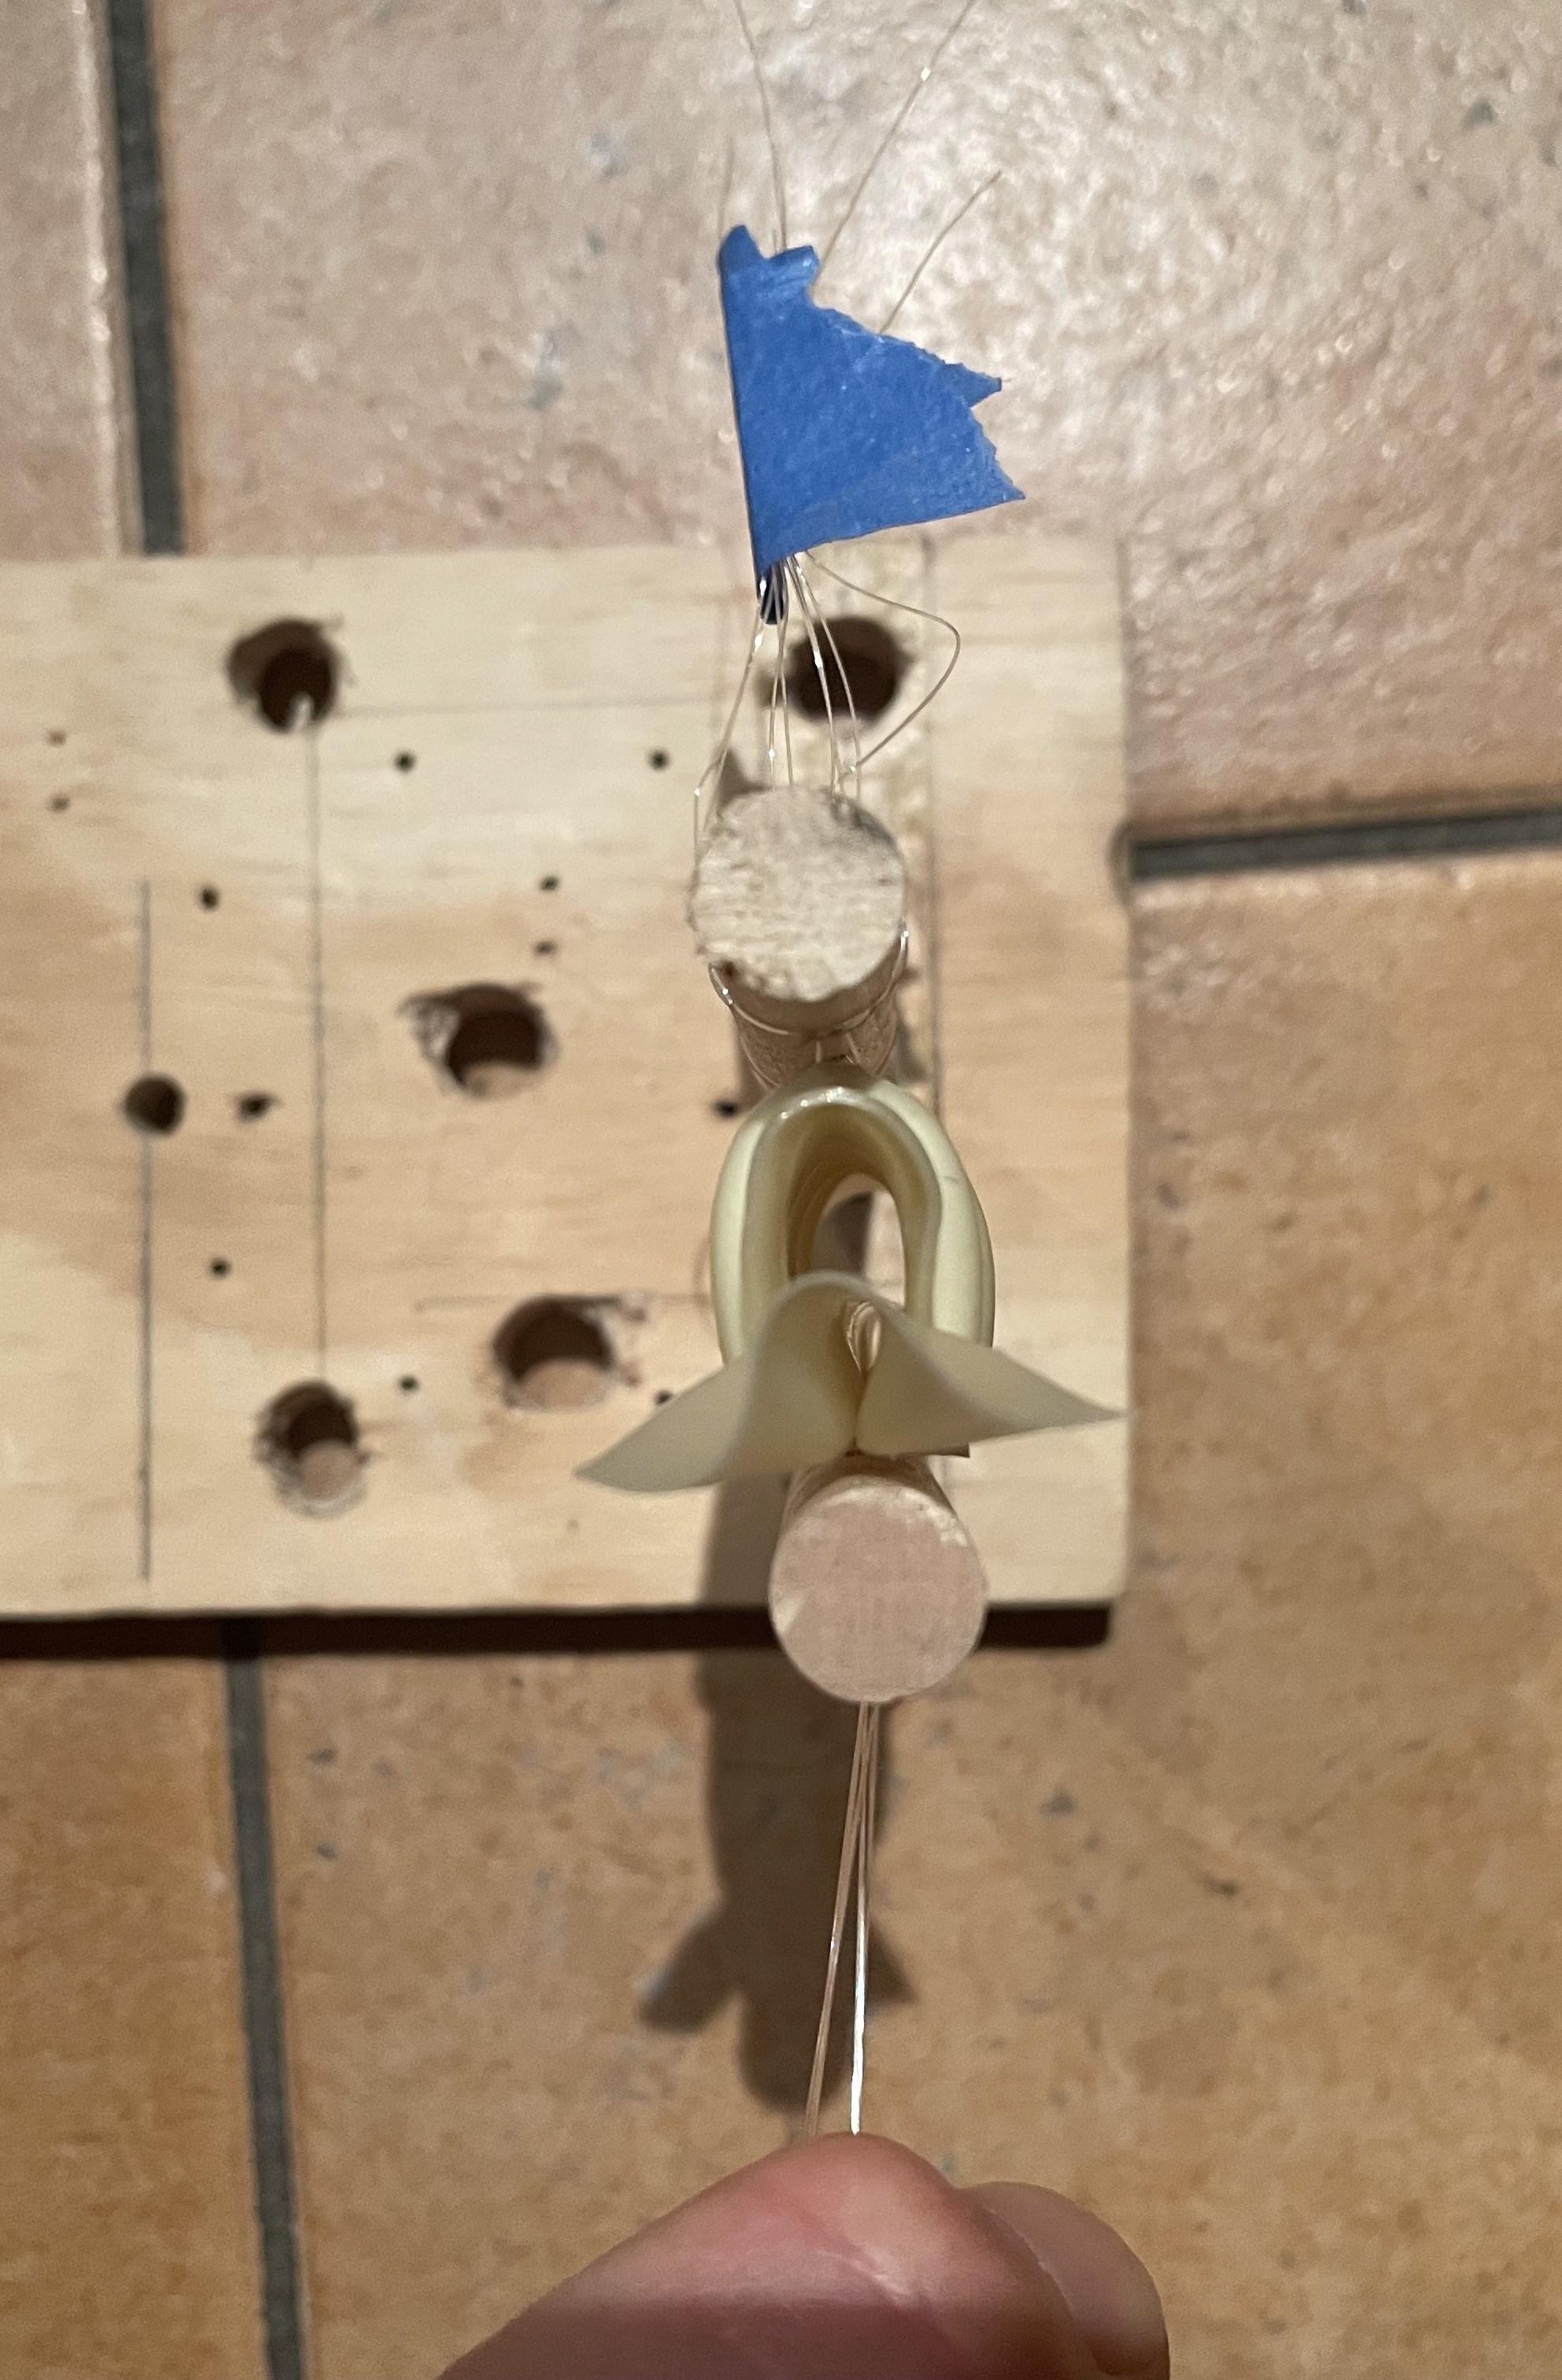
\includegraphics[width=0.22\textwidth]{images/49.JPG}
  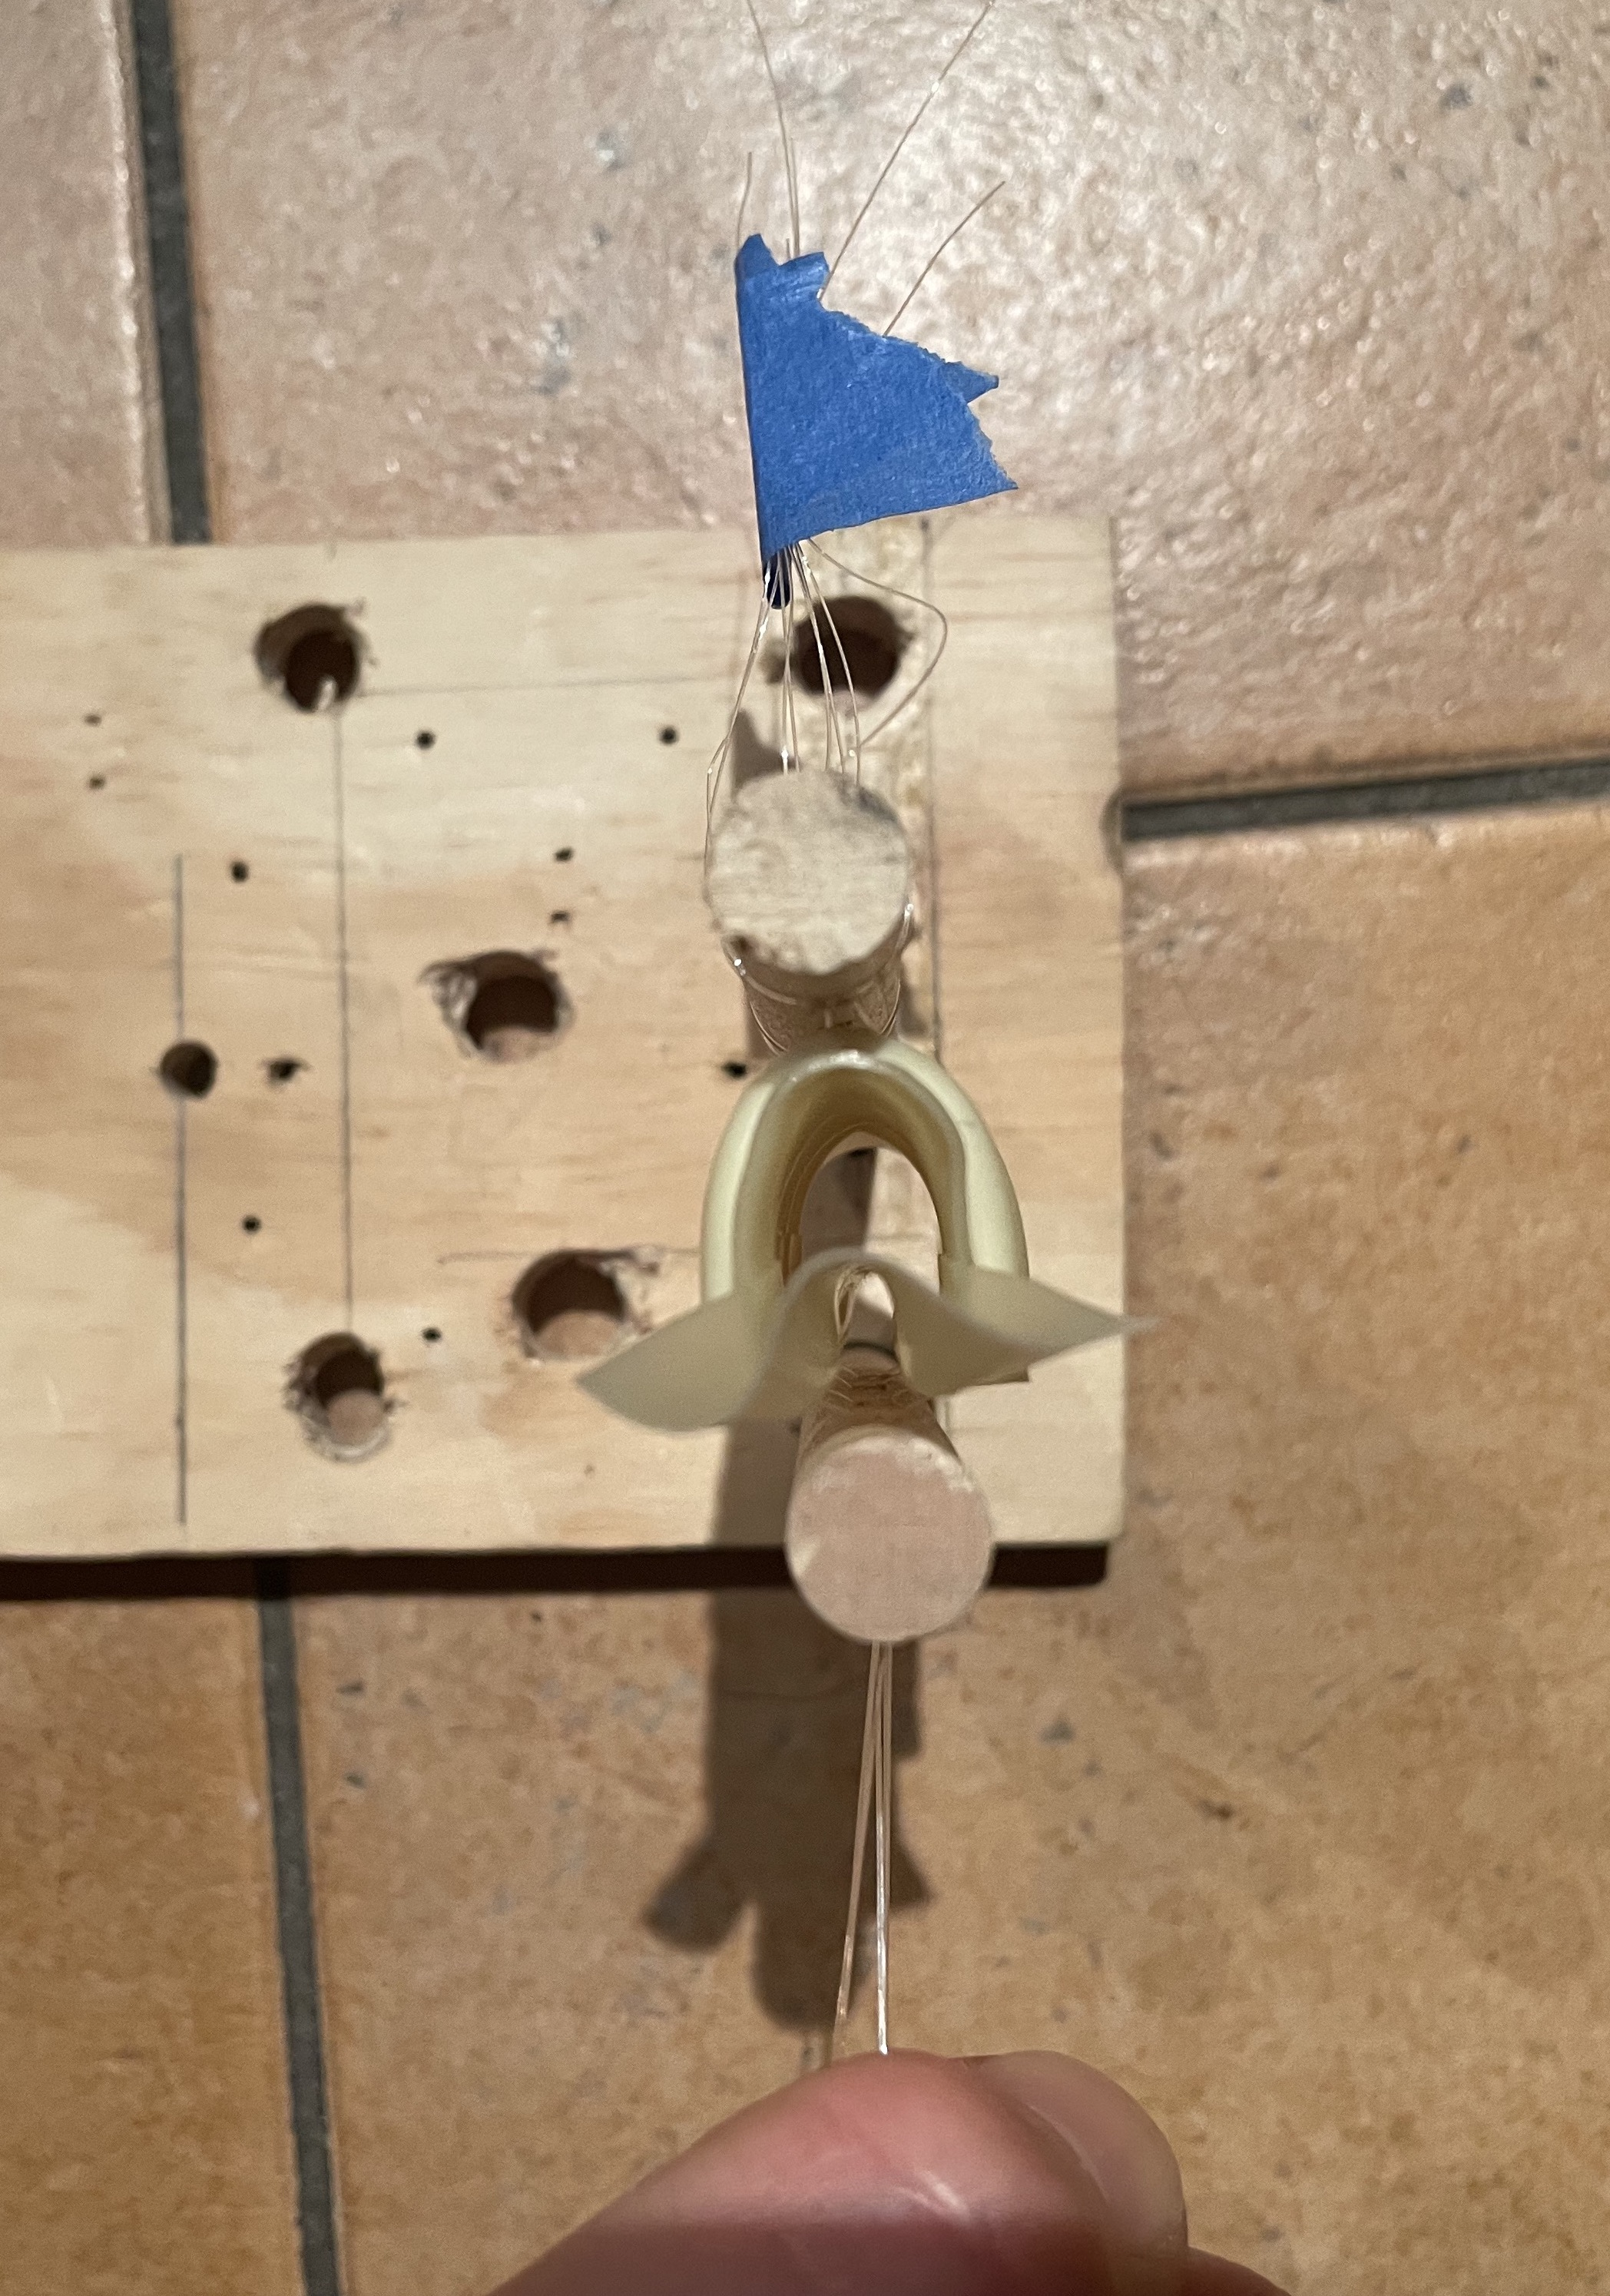
\includegraphics[width=0.22\textwidth]{images/50.JPG}
  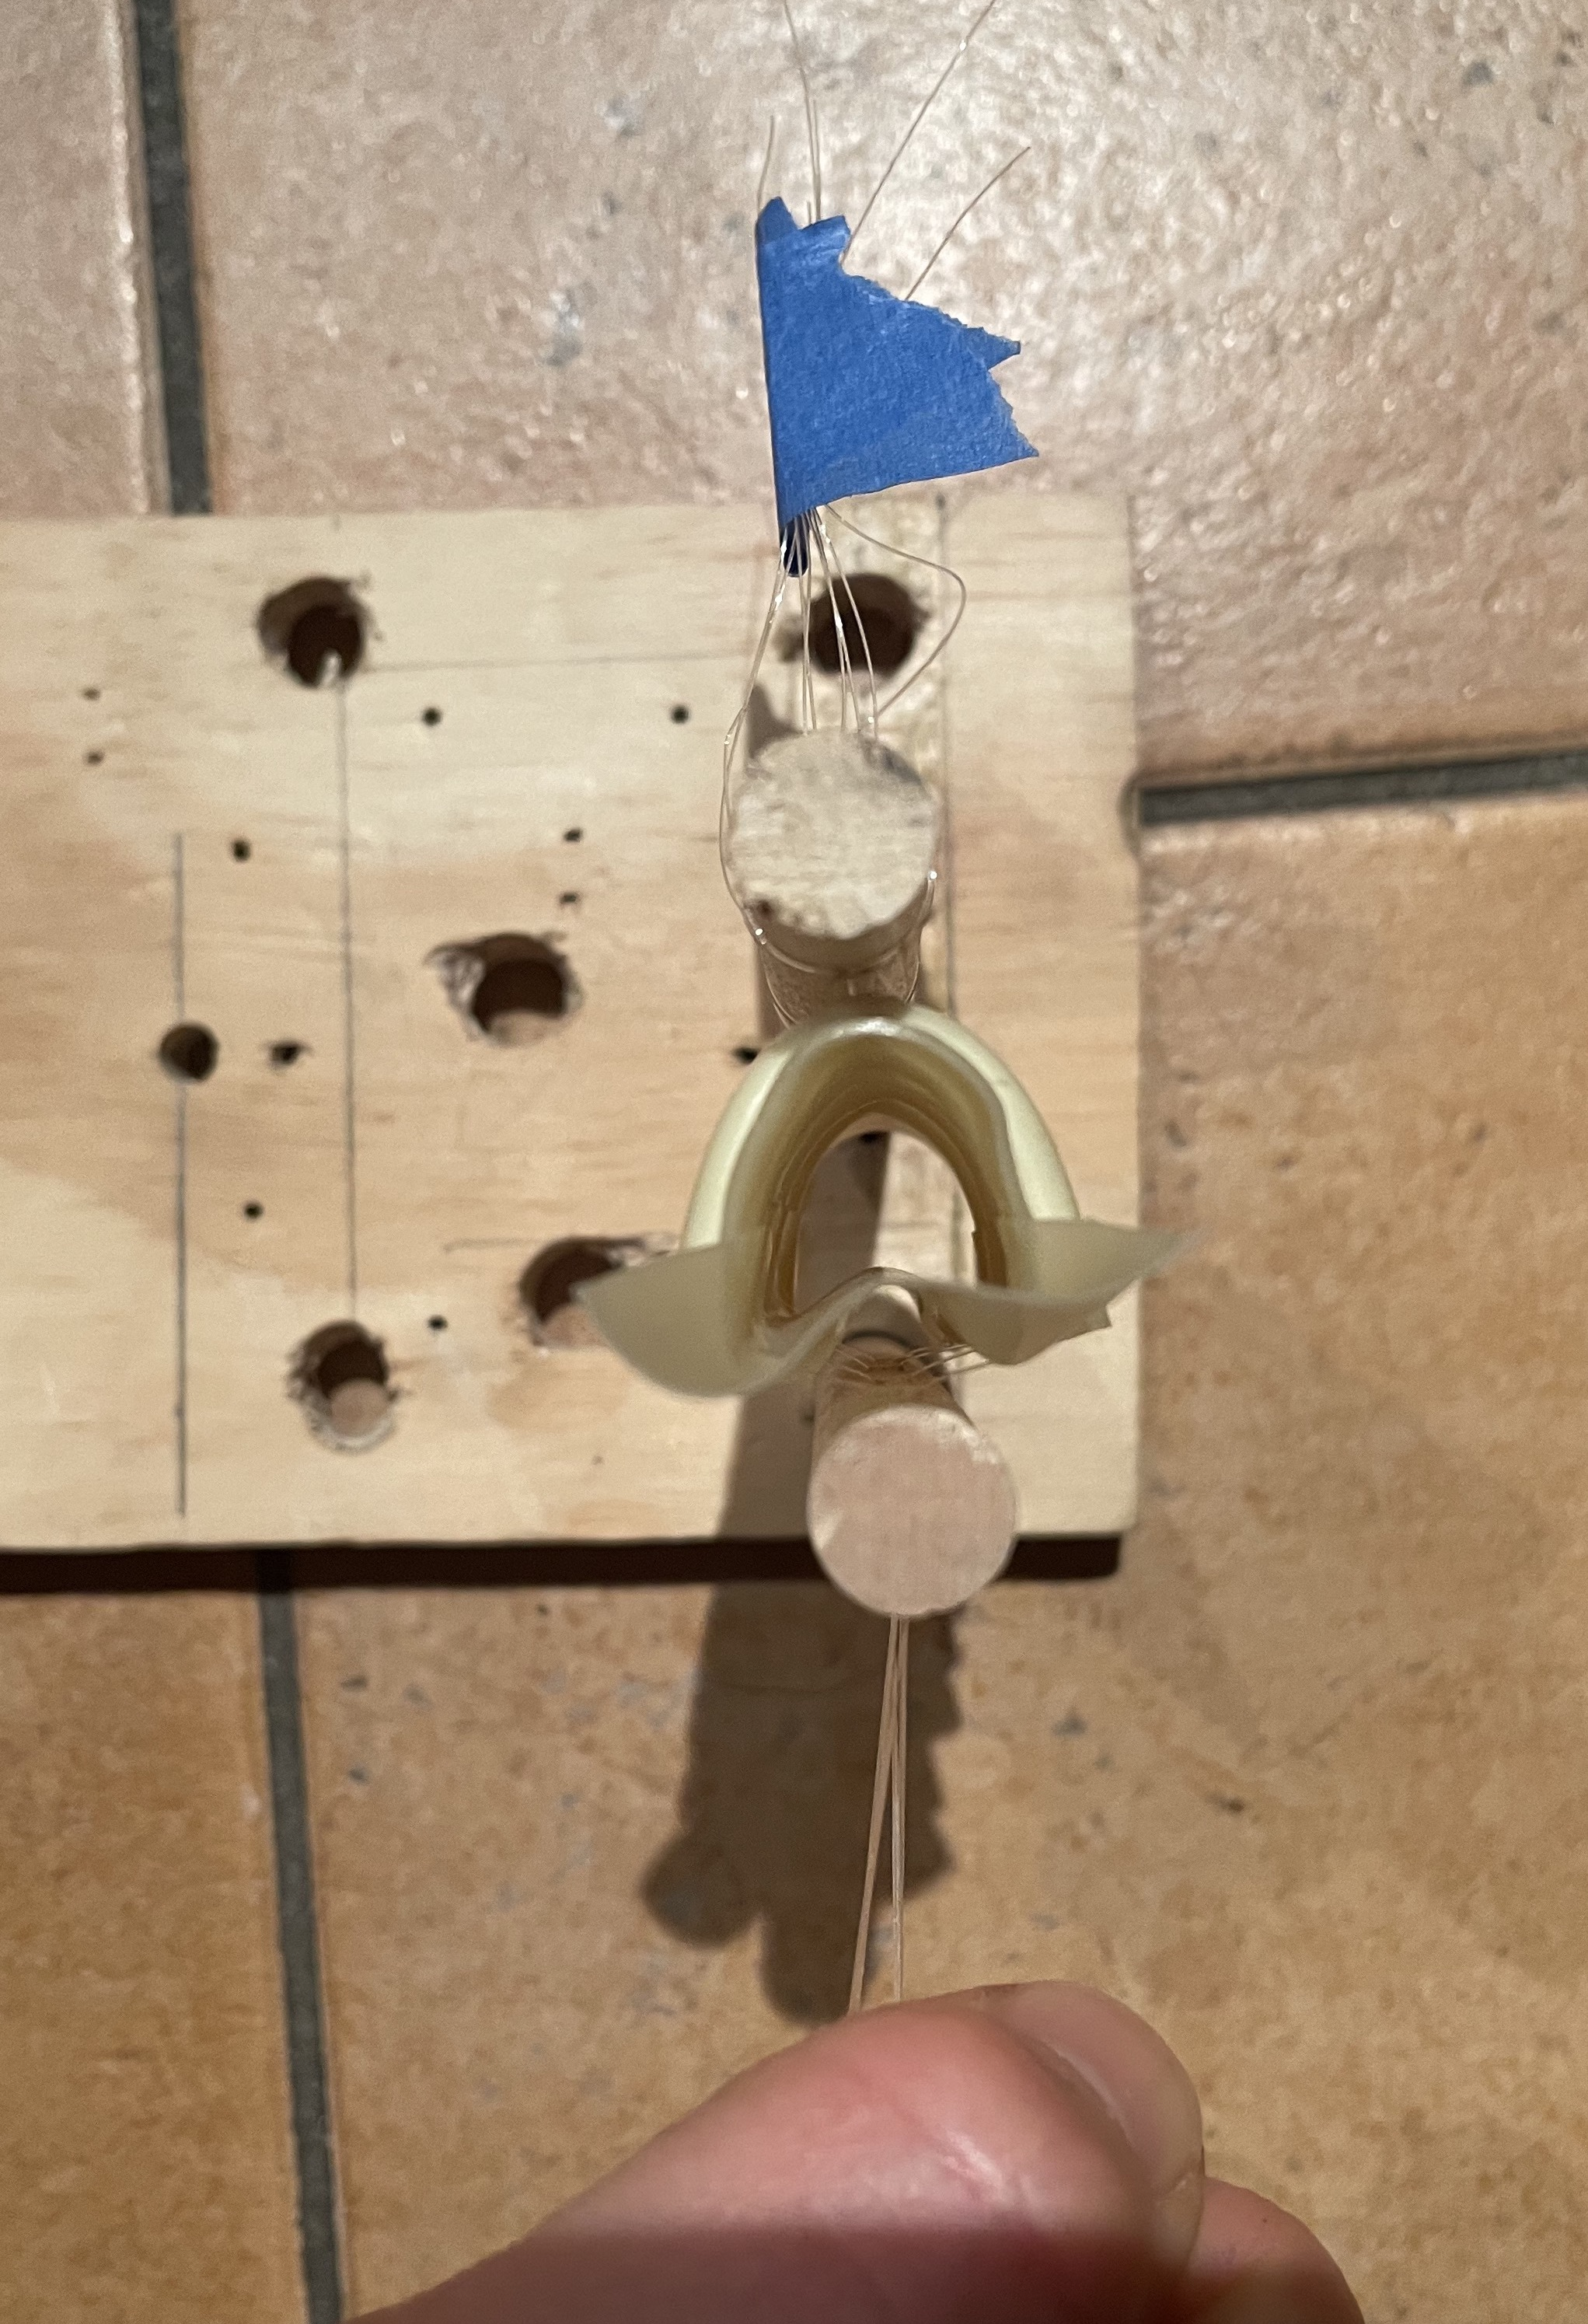
\includegraphics[width=0.22\textwidth]{images/51.JPG}
  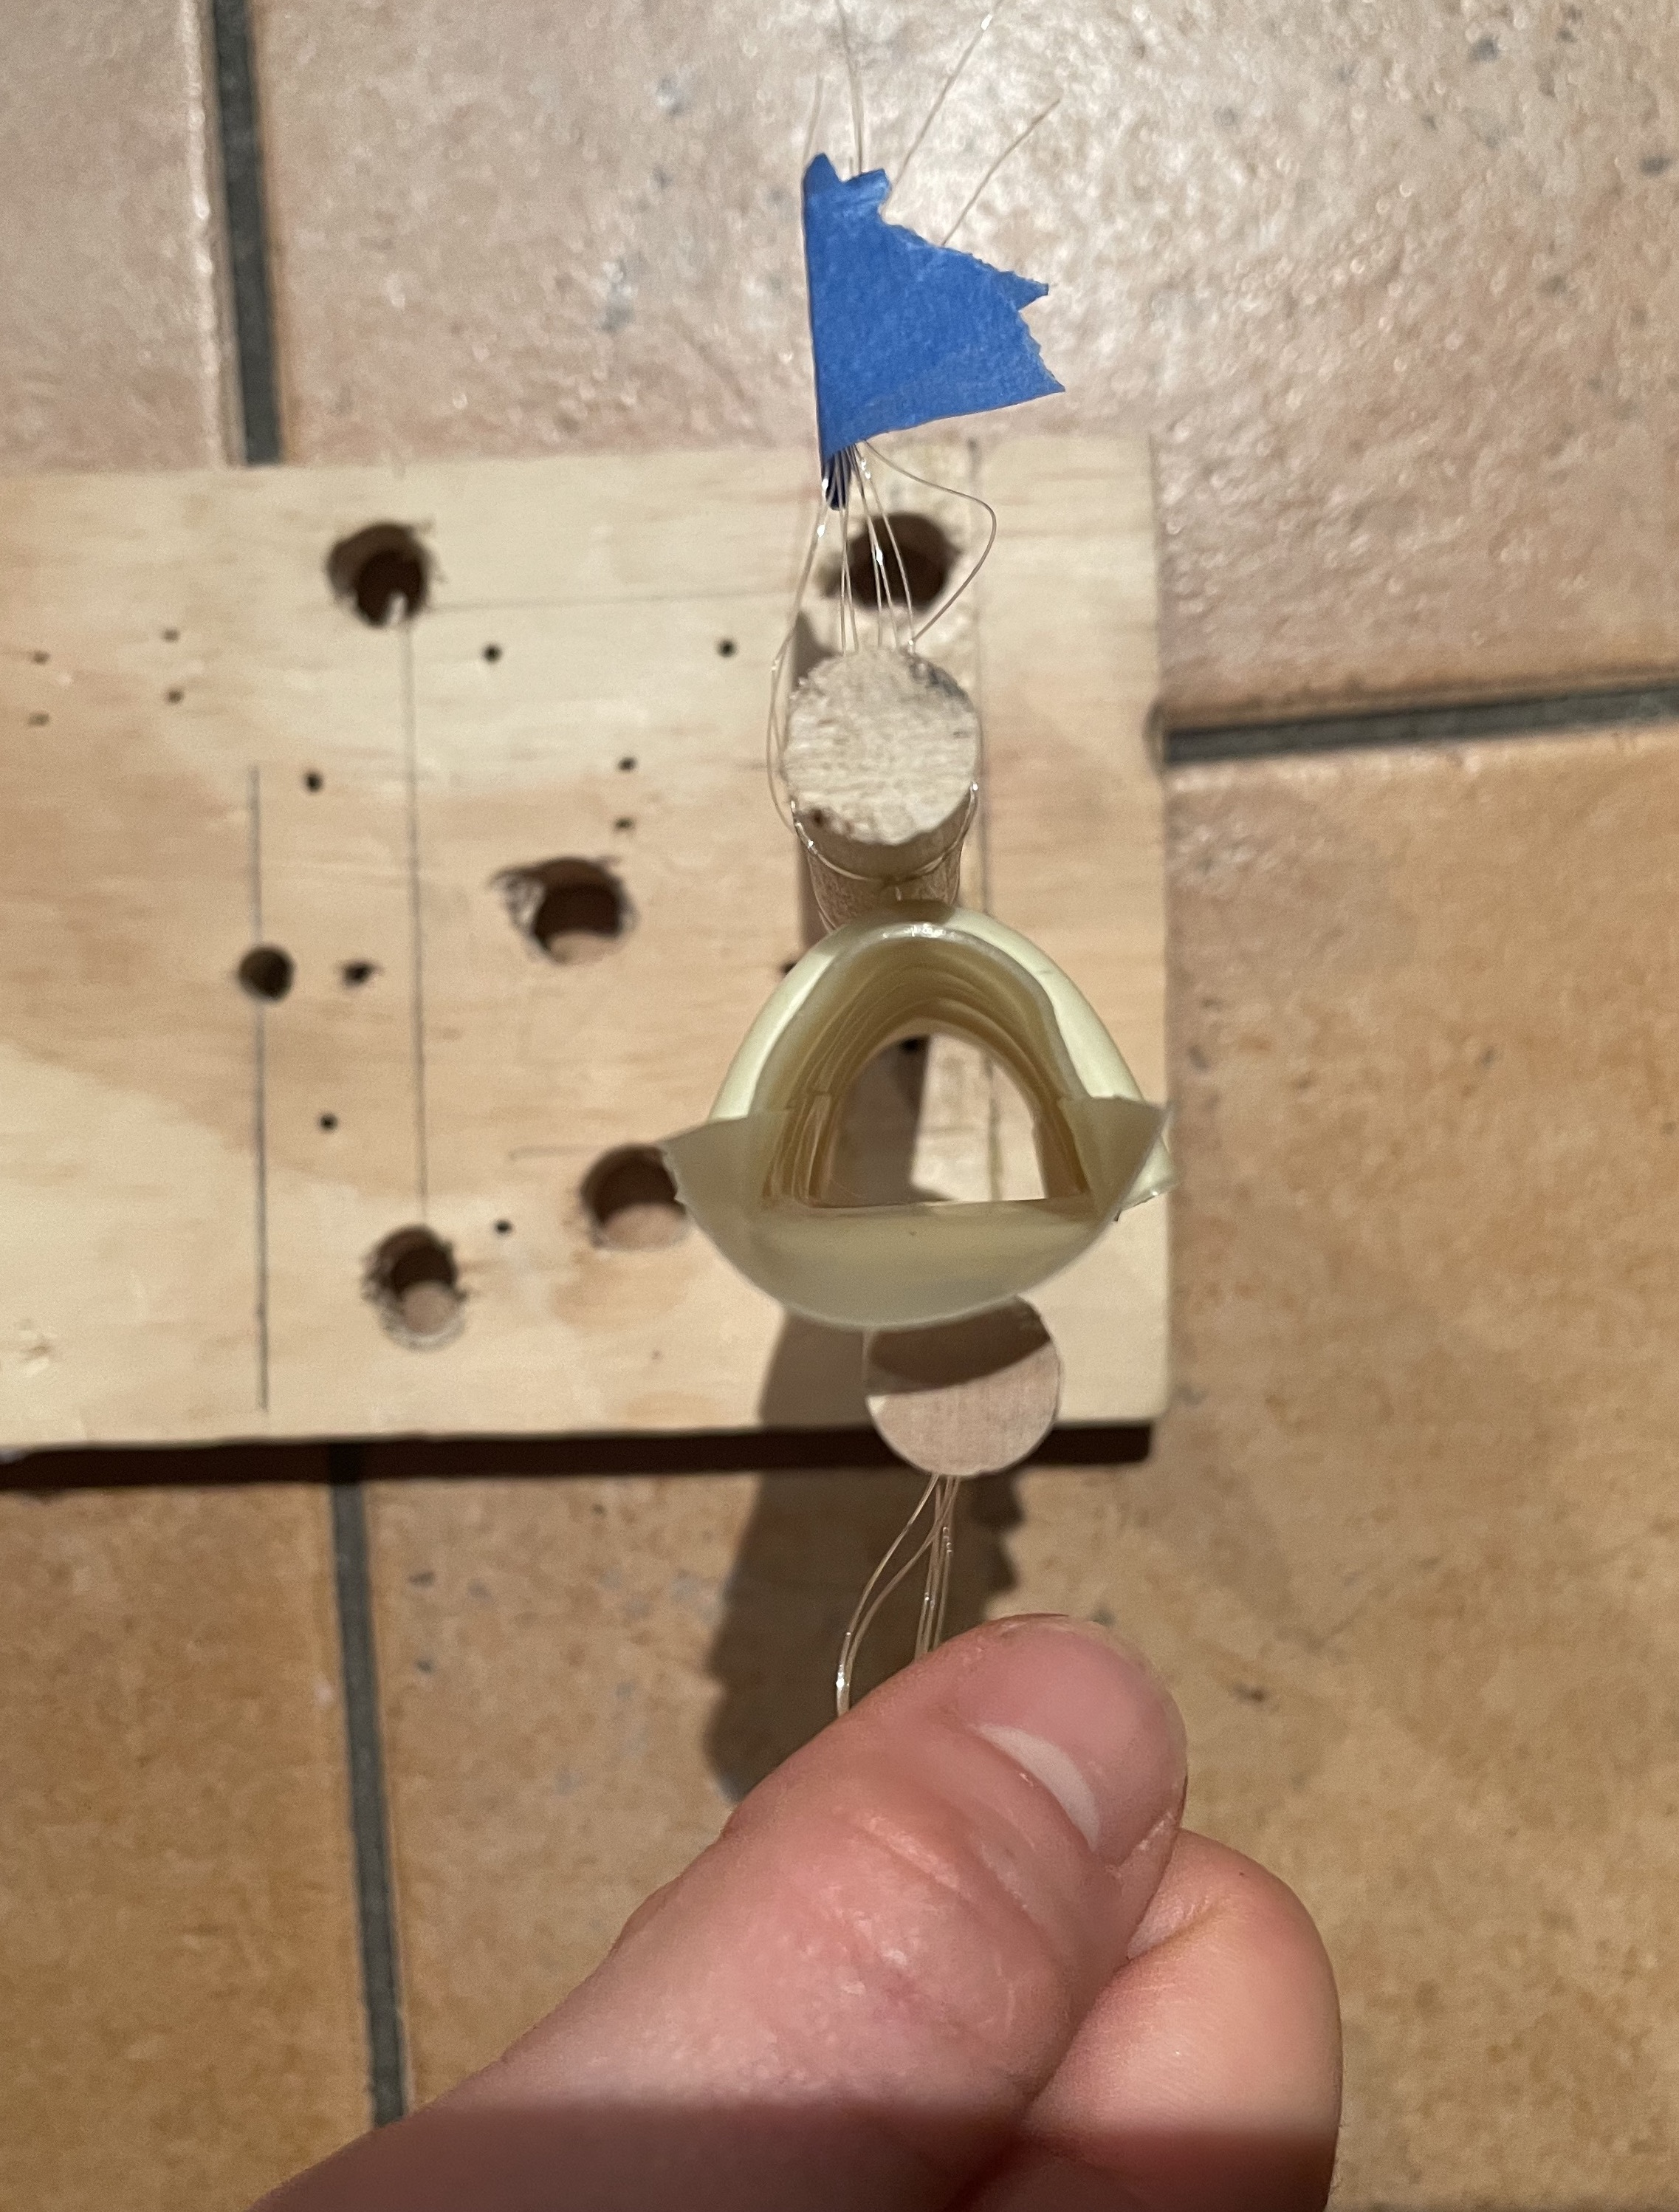
\includegraphics[width=0.22\textwidth]{images/52.JPG}
  \caption{sequence of contracting each ring then releasing all of them slowly}
\end{figure}


Takeaways:
\begin{itemize}
\item
it's important to use a sharp needle when going through latex cause it's really stretchy
\item
I need to get this in a position so I can move air through it!
\item
  this works really well for something that's 3" long, but I'll need to use something that's much more ridgid for the 
\end{itemize}
\clearpage
\subsection*{four (11/03/2021)}
\textbf{name:} latex / trachea trial no. 2

\textbf{soundtrack:} Gillian Welch discography all day (every couple months I spend one day listening to all her music) 

The intent of this prototype was to see how close to a trachea structure I could get. I repeated the same experiemnt from Tuesday night more carefully and with more components in a nattempt to construct ad better trachea protptype. The goal was to create a closed tube with a mechanism in place to create a change in shape.

First I carefully cur my pieces of latex to size -- two 3" x 1.5" pices. Then I cut four pieces of vinyl tubing to 1.5" lengths to embed in the latex. I cleaned and prepared the latex with glue, then sandwiched the vinyl tubing between the latex pieces. I used a pretty thin and even layer of glue and was very careful to prevent air bubbles. 

Next I took another 1.5" wide piece of latex and applied glue to the edge. I applied glue to one edge of my tubing assembly and after waiting the appropriate aount of time, carefully stuck the two edges together with about 1/4" of overlap. 

The next step -- closing the tube -- was tricky. To prevent the vinyl tubing from pulling apart the new seams I took pieces of wire and threaded them through the tubing. Then I bent them into a U shape keeping the twp sides I waas gluing close together with little tension on them. I then applied glue to the other side of the sandwich andt he other isde of the flap and sealed the other side. 

After letting this sit for some time, I began to remove the wire pieces and replace them with bits of monofilament like in the previous prototype. I was pleasantly surprised by how well the glue sustained the tension from the vinyl tubing. Nothing began to tear or separate sinificantly, though there was one spot that looked like it didn't get enough glue.


Things I learned:
\begin{itemize}
\item
  this was pretty a easy easy with a 3" section, but I think it will be more difficult with a longer tube
\item
  the latex to latex bond is pretty strong and didn't come apart from the pressure of the viny tubing
\item
  I need to think of a clever way to mount this so that it can be mechanised
\item
  I ended up skimming a cool medical paper about breath noises while making this prototype...need to revisit BUT the gist was that the brachea and trachea are the really important parts of breath noises. The coolest thing I learned -- aside from a bunch of laminar flow stuff in the lungs -- is that our organs and chest stuff act as a low pass filter for noises coming from our lungs and lower brachea / trachea. Most of the higher frequency breath noises that we hear come from the neck where there's less tissue for the sound to travel through. Waves! Definitley need to read more thoracic medicine papers.
\end{itemize}

\clearpage
\section*{nothing (11/02/2021)}

Had to do work work for my job instead.


\clearpage
\section*{three (11/01/2021)}
\textbf{name:} latex trial no. 1

\textbf{soundtrack:} my own breath in a respirator

This prototype is also going to span multiple days and build on itself. The intent of this first try was to get a feel for working with latex. 

First I assembled my materials. A few 2" x 2" squares of 14 mil latex, some rubbing alchohol, and a bottle of rubber cement. Then I prepared my work area, which was a little tricky since the window in my studio wouldn't open. I ended up working on top of the stove with the vent hood on while weraing a respirator.

After reading a little bit on the internet I went for it. The order of operations is to put glue on both pieces of latex, let it dry for about 5 minutes and then stick the two together. When you put the glue on initially the latex shrivels up. As time passes it relaxes and returns to its original shape. Even though I expected this I was pretty surprised to see just how much it shrivled. I wasn't really sire about the rubbing alchohol so I left it out at first. 

The first test I did turned out well, all things considered. The two pieces of latex were firmly stuck together. While the latex was relaxing I started watching a youtube video for more instruction. Even though I hate instructional youtube videos, this one was quite helpful. I learned that I was using too much glue and that it's a good idea to wipe the latex with rubbing alchohol before applying glue, as I suspected.

For the second test I used a q-tip and first wiped the gluing area with isopropyl. Then, using another q-tip I applied a much thinner layer of glue than before. The latex still curled up, but it was less messy and uncurled faster. I was also more mindful to avoid air bubbles as I stuck the two pieces together. This test went pretty well, but still had a lot of air bubbles and wasn't very flat.

For the last test I decided to embed two small pieces of vinyl tubing between the sheets of latex to play with changing the shape of the sheet. I applied the glue as usual and then once it had dried set the two pieces of tube on the glue side oasdf one piece. I then carefully applied the other piece of glue latex. This time I was veyr mindful not to get any airbubbles and the final result was quite smooth. Its appearnce is certainly reminiscent of ridged tissue with cartalidge.

Then I threaded some monofilament through the tube and some glass beads I found in the dryer with my laundry -- the fact that I can always seem to find the materials I need, but not my fancy new bike sock is irksome but feels fair -- and played around. Without a structure to hold the tube it was tricky to contract it. 



Things I learned and new questions to address:
\begin{itemize}
\item
the british guy on youtube said you should only work with a small vessel of gue and isopropyl at a time to minimize evaporation...need to find some tiny jars
\item
need to determine how strong the bond is -- how could I create an anchor point needed to mechanize the diaphragm?
\item
my experiement with the vinyl tubing is cool, but it would be better if the vinyl formed a closed tube and the whole thing was more mechnically robust
\item
what sounds or feeling does water have on the latex?
\item
I continue to have a slight allergy to latex powder. Hopefully it doesn't get worse. I will find nitrile gloves and continue not to touch my face.
\item
...more questions to come
\end{itemize}


\clearpage
\section*{two (10/31/2021)}

\textbf{name:} disembodied breath no. 1

\textbf{soundtrack:} some of Mirrors by Angel Olsen and Late Night Feelings by Mark Ronson et. al ...piecemeal listening today

This prototype is defintely going to span two days. Today being Halloween seemed like an appropriate day to start, however.

The goal of this prototype is to understand the response to the sound of disembodied breath. To achieve this will use my trusty buckets to "produce" breath sounds. I would say that this prototype is Wizard of Oz adjacent.

Fist I took a small bluetooth speaker and the biggest USB battery I have. I made sure that they fit inside one 5 gallong bucket when another was placed on inside. 

Then I put the bucket from yesterday with the hole and latex tube attached inside the bucket with the speaker. 

I connected to the speaker with my cellphone and played a youtube video of breath noises at a loud volume. It was a very striking effect.

I took my buckets -- the new, hottest trend in streetwear accessories -- out on the street and found a cafe on a pretty busy corner. I put them on the sidewalk and played breath noises.

A number of things went wrong; I needed to use my cellphone for something other than youtube, the bluetooth kept disconnecting, and due to street noise and music from the cafe no one really heard the bucket. I also placed it near a trash can and was worried someone would throw something yucky inside.

Then I went home and created an mp3 from the youtube video. I put it on an old cellphone on repeat and used an aux cable to connect the speaker to the cellphone. 

Sometime later I took this, much more solid, combination out to my favorite corner bar with my sister who was visiting. And placed it near a crosswalk (the same one I used for instruction sets for strangers, in fact).

Not too many people noticed the bucket. I think the road noise was a lot to contend with. The people that did notice were pretty funny. Three interactions stand out:
\begin{itemize}
\item
A young woman kept looking at the bucket while waiting for the crosswalk with a group of friends. She kept looking furtively over her shoulder at the bucket and was clearly perturbed by the noise. It was also clear from her interaction walking away that she didn't immediately mention it to her companions. 
\item
A man in his late 50s perhaps was eating a slice of pizza while crossing the street. When he got to the bucket he stopped and was very curious. He looked inside and listened closely. He clearly wasn't in a rush as he finished his pizza. Throughout the interaction his facial expression was a mix of confusion, disgust and laughter. He walked away shaking his head. 
\item
A young man was smoking a cigarette near the bucket. After some time he started looking at it more closely and clearly noticed the sound. He seemed confused and a bit disconcerted. My sister and I were clearly looking at him so he came over to us and mentioned that he though someone had ``planted something" on the corner. He said he'd thought it was music and had been waiting for a pop song to start playing, but nothing happened. 
\item
Finally, a woman collecting recycling walked by. She stopped at the trash can adjacent to the bucket. And then I watched in seeminly slow motion as her attention turned to my prized buckets. She seemed a bit confused, but bent over and took the inner bucket out. At that point I left my seat and went over and asked her to stop. I explained that the buckets were mine and she apologized and went on her way. Then it was time ot go home.
\end{itemize}

The big takeaways which I want to adjust on the next iteration aere as follows:
\begin{itemize}
\item
needs to be louder
\item
needs a more quiet location
\item
need a better way to control which breath sounds are playing
\end{itemize}

To account for these, I think I'm going to try a park. I can't find a louder speaker, but maybe I can make the noise louder digitally. I am also going to create simple interface which will let me adjust which breath sounds are playing instead of having to listen to the youtube video mp3 on repeat.
\clearpage
\subsection*{one (10/30/2021)}

\textbf{name:} diaphgarm test no. 1

\textbf{soundtrack:} Treehouse by Sofi Tukker

The objective of this prototype was to create a mechanism for forcing air through a tube so that I can play with different sounds. To do this I intended to create a diaphragm to move the air. My intention was to attach a pice of latex over one end of the bucket and a small tub at the other.

I started with one of the 5 gallon buckets I found and bought a bucket lid (should've tried harder to find the lids when I found the buckets).

I cut the center out of the lid and then did a test to see how well the latex stayed in place under the lid. Luckily it worked well and didn't damage the latex.

Next, I drilled a hole in the bottom of the bucket. I forgot about my hole saw kit and just used a knife to slowly shave off the edges until it was the right size for the tube.

Then I trimmed a pice of Latex to size (this required a fresh box cutter since all my other knives were too dull for a clean cut).

Finally, I attached the latex to the open end of the bucket under the "lid" and poked the tub through the hole in the bottom.

The effect was pretty immediate. By depressing the diaphragm I easliy forced air out through the tube -- an exhale -- and air came back into the tube when I let the diaphragm rebound -- inhale. 

There were three pnysical properties I wanted to play with to see how they impacted the sound coming from the prototype:
\begin{enumerate}
\item
how much of the tube was outside of the bucket vs. inside
\begin{itemize}
\item
This didn't seem to have a big impact. It was really ahrd to tell the difference between the tube being all the way out and all the way in. I think I need to cut the tube ot be different lengths.
\end{itemize}
\item
how sound changed when the tube was pinched in different places
\begin{itemize}
  \item
    when the tube was pinched near the bottom the sound was lower in pitch
  \item
    when the tube was pinched near the top the sounds was higher in pitch
  \item
    nearer the top sounded more like human breathing
\end{itemize}
\item
how sounds changed if the bucket was crushed sideways to be less round
\begin{itemize}
  \item
    this one was also hard to tell, it seemed that there was slighly less resonance when the bucket was crushed
  \item
    the intent was to make the sound less hollow and I think this was slightly true
\end{itemize}

\end{enumerate}

\vspace{1cm}
I think this prototype was pretty successful. It left me with a good number of questions which are as follows.
\begin{itemize}
\item
  how does the length of the output tube effect the sound? need to experiement, but an not ready to cut the tube.
\item
  how does the shape of the cavity effect the sound?
\item
  is this cavity ridiculously large in comparison to normal lungs?
\item
  how do I make the sound less hollow?
\item
  what volume of air is displaced? (if I had a flow meter I could just integrate, but I'll have to be more clever)
\item
  how would a lung structure change the sound?
\item
  how would the sound change if there was some kind of foam or cloth inside the cavity? would that sound less hollow?
\item
  how the heck am I going to automate the diaphragm?
\end{itemize}

\clearpage
\section*{7 in 7 planning}

The first step of any prototyping exercise is to collect materials. I did some of this a couple weeks ago when I went to canal rubber (so cool, so much sneezy latex powder). This was good fodder for the diaphragm and trachea prototypes, but I still need a chest cavity like thing that would be more robust than the small plastic container I tried already. A large plastic carboy for brewing would be ideal, but that violates my prototyping rule of only buying things you truly need for a material or functional evaluation (like latex) and can't find anywhere else. While out on a late walk this Monday evening I found a lot of recycling outside a restaurant near my apartment. Isolated inside a single clear trashbag were three 5 gallon buckets formerly containing pickles. These streets deliver! They didn't even smell much like pickles once I got them home and opened the bag. After a few days outside and a big rainstorm they were good to go. Seems like I already have the necessary materials for my other physical protptypes. 

\subsection*{proposed prototypes}

There are two sensory aspects of this work, the auditory and the physical or visual. It was pretty easy to identify prototypes that fell in each of these categories. The auditory prototypes should play with differnet types of breath and evaluate the effect of disembodied breath. The physical prototype should focus solely on the mechanical aspec of reproducing breath according to the basic breakdown of the respiratory system I've outlined. I'm not going to start thinking about the electronics used to actuate the thigns.
%outside of investigating what might be quiet.

It was less easy to think about prototypes that address the less tangible questions I am hoping to probe with this work. To think about this I started by looking back at the questions I asked myself originally. After reviewing that list, the big question I want to start asnwering is how a viewer sees their own presesnce near the work impacting its breath. This is an answer to the questions of who holds power over our own breath and how far does breath extend as a metaphor for out relationship with the natural world. I'm going to start with this one isolated question because it has a lot of facets and ultimately will lead to the bigger question of what should the viewer take away from the work (in other words, what experience do I intend for them to have). 

Based on the above thinking I concoted the following protptypes.


%What if as more people enter a space, or come closer to the contraption, it becomes more difficult for it to breath?

\vspace{1 cm}
\textbf{interactive (how a viewer sees their own presence near the work impacting its breath):}

as someone approaches the bucket the breath becomes worse

as someone leaves the bucket breath becomes worse

breath eminates from a tree? that's a bit random, but perhaps illustrative

\vspace{1 cm}
\textbf{auditory (addressing disembodied breath, how breath denotes sickness, difficulty, and emotion):}

Hide a speaker and battery inside two 5 gallon buckets in a public place with moderate traffic and see how people react. Do each of these different types of breath illicit different reactions?

play normal breath sounds 

play laboured and sick (covid equivalent) breath sounds

play emotional breath sounds (sad, happy, aroused, etc.)


\vspace{1 cm}
\textbf{visual / physical (addressing how to actually make this thing and how it should look):}

make a big diaphragm and play with \textit{quiet} ways to make it move

make a trachea protptype with multiple rings that contract

play with the idea of a larynx

model a brachea in openSCAD and print one small piece to think about how moitsure could interact with this piece


\end{document}
